\documentclass[11pt,preprint, authoryear]{elsarticle}

\usepackage{lmodern}
%%%% My spacing
\usepackage{setspace}
\setstretch{1.2}
\DeclareMathSizes{12}{14}{10}{10}

% Wrap around which gives all figures included the [H] command, or places it "here". This can be tedious to code in Rmarkdown.
\usepackage{float}
\let\origfigure\figure
\let\endorigfigure\endfigure
\renewenvironment{figure}[1][2] {
    \expandafter\origfigure\expandafter[H]
} {
    \endorigfigure
}

\let\origtable\table
\let\endorigtable\endtable
\renewenvironment{table}[1][2] {
    \expandafter\origtable\expandafter[H]
} {
    \endorigtable
}


\usepackage{ifxetex,ifluatex}
\usepackage{fixltx2e} % provides \textsubscript
\ifnum 0\ifxetex 1\fi\ifluatex 1\fi=0 % if pdftex
  \usepackage[T1]{fontenc}
  \usepackage[utf8]{inputenc}
\else % if luatex or xelatex
  \ifxetex
    \usepackage{mathspec}
    \usepackage{xltxtra,xunicode}
  \else
    \usepackage{fontspec}
  \fi
  \defaultfontfeatures{Mapping=tex-text,Scale=MatchLowercase}
  \newcommand{\euro}{€}
\fi

\usepackage{amssymb, amsmath, amsthm, amsfonts}

\def\bibsection{\section*{References}} %%% Make "References" appear before bibliography


\usepackage[round]{natbib}

\usepackage{longtable}
\usepackage[margin=2.3cm,bottom=2cm,top=2.5cm, includefoot]{geometry}
\usepackage{fancyhdr}
\usepackage[bottom, hang, flushmargin]{footmisc}
\usepackage{graphicx}
\numberwithin{equation}{section}
\numberwithin{figure}{section}
\numberwithin{table}{section}
\setlength{\parindent}{0cm}
\setlength{\parskip}{1.3ex plus 0.5ex minus 0.3ex}
\usepackage{textcomp}
\renewcommand{\headrulewidth}{0.2pt}
\renewcommand{\footrulewidth}{0.3pt}

\usepackage{array}
\newcolumntype{x}[1]{>{\centering\arraybackslash\hspace{0pt}}p{#1}}

%%%%  Remove the "preprint submitted to" part. Don't worry about this either, it just looks better without it:
\makeatletter
\def\ps@pprintTitle{%
  \let\@oddhead\@empty
  \let\@evenhead\@empty
  \let\@oddfoot\@empty
  \let\@evenfoot\@oddfoot
}
\makeatother

 \def\tightlist{} % This allows for subbullets!

\usepackage{hyperref}
\hypersetup{breaklinks=true,
            bookmarks=true,
            colorlinks=true,
            citecolor=blue,
            urlcolor=blue,
            linkcolor=blue,
            pdfborder={0 0 0}}


% The following packages allow huxtable to work:
\usepackage{siunitx}
\usepackage{multirow}
\usepackage{hhline}
\usepackage{calc}
\usepackage{tabularx}
\usepackage{booktabs}
\usepackage{caption}


\newenvironment{columns}[1][]{}{}

\newenvironment{column}[1]{\begin{minipage}{#1}\ignorespaces}{%
\end{minipage}
\ifhmode\unskip\fi
\aftergroup\useignorespacesandallpars}

\def\useignorespacesandallpars#1\ignorespaces\fi{%
#1\fi\ignorespacesandallpars}

\makeatletter
\def\ignorespacesandallpars{%
  \@ifnextchar\par
    {\expandafter\ignorespacesandallpars\@gobble}%
    {}%
}
\makeatother

\newenvironment{CSLReferences}[2]{%
}

\urlstyle{same}  % don't use monospace font for urls
\setlength{\parindent}{0pt}
\setlength{\parskip}{6pt plus 2pt minus 1pt}
\setlength{\emergencystretch}{3em}  % prevent overfull lines
\setcounter{secnumdepth}{5}

%%% Use protect on footnotes to avoid problems with footnotes in titles
\let\rmarkdownfootnote\footnote%
\def\footnote{\protect\rmarkdownfootnote}
\IfFileExists{upquote.sty}{\usepackage{upquote}}{}

%%% Include extra packages specified by user
\usepackage{booktabs}
\usepackage{caption}
\usepackage{longtable}

%%% Hard setting column skips for reports - this ensures greater consistency and control over the length settings in the document.
%% page layout
%% paragraphs
\setlength{\baselineskip}{12pt plus 0pt minus 0pt}
\setlength{\parskip}{12pt plus 0pt minus 0pt}
\setlength{\parindent}{0pt plus 0pt minus 0pt}
%% floats
\setlength{\floatsep}{12pt plus 0 pt minus 0pt}
\setlength{\textfloatsep}{20pt plus 0pt minus 0pt}
\setlength{\intextsep}{14pt plus 0pt minus 0pt}
\setlength{\dbltextfloatsep}{20pt plus 0pt minus 0pt}
\setlength{\dblfloatsep}{14pt plus 0pt minus 0pt}
%% maths
\setlength{\abovedisplayskip}{12pt plus 0pt minus 0pt}
\setlength{\belowdisplayskip}{12pt plus 0pt minus 0pt}
%% lists
\setlength{\topsep}{10pt plus 0pt minus 0pt}
\setlength{\partopsep}{3pt plus 0pt minus 0pt}
\setlength{\itemsep}{5pt plus 0pt minus 0pt}
\setlength{\labelsep}{8mm plus 0mm minus 0mm}
\setlength{\parsep}{\the\parskip}
\setlength{\listparindent}{\the\parindent}
%% verbatim
\setlength{\fboxsep}{5pt plus 0pt minus 0pt}



\begin{document}



\begin{frontmatter}  %

\title{Question 3: Portfolio Construction}

% Set to FALSE if wanting to remove title (for submission)




\author[Add1]{Jan-Hendrik Pretorius}
\ead{20713479@sun.ac.za}





\address[Add1]{Stellenbosch University}


\begin{abstract}
\small{
This report examines the methodologies and performance of the ALSI
(J203) and SWIX (J403) Indexes, analyzing differences in returns across
market capitalizations, sector exposures, and stock concentrations. It
also assesses the impact of currency performance and volatility on these
indices and considers the implications of applying different capping
thresholds during quarterly rebalances. The findings reveal distinct
return profiles between the indexes and offer insights into the effects
of capping on market representation and performance.
}
\end{abstract}

\vspace{1cm}





\vspace{0.5cm}

\end{frontmatter}

\setcounter{footnote}{0}



%________________________
% Header and Footers
%%%%%%%%%%%%%%%%%%%%%%%%%%%%%%%%%
\pagestyle{fancy}
\chead{}
\rhead{Question 3: Portfolio Construction}
\lfoot{}
\rfoot{\footnotesize Page \thepage}
\lhead{}
%\rfoot{\footnotesize Page \thepage } % "e.g. Page 2"
\cfoot{}

%\setlength\headheight{30pt}
%%%%%%%%%%%%%%%%%%%%%%%%%%%%%%%%%
%________________________

\headsep 35pt % So that header does not go over title




\hypertarget{performance-analysis}{%
\section{Performance Analysis}\label{performance-analysis}}

The figure below presents a multi-faceted view of the ALSI J203 Index
returns, segmented by market capitalization categories: Large-Caps,
Mid-Caps, and Small-Caps. The top-left panel shows the cumulative
returns, where Large-Caps exhibit a significant upward trend, greatly
outperforming the other categories. The top-right panel illustrates
drawdown periods, with all categories showing similar drawdowns,
indicating that market downturns affect all capitalizations fairly
equally. The bottom-left panel shows rolling returns, calculated on an
annual basis, with Large-Caps demonstrating less volatility and more
stable returns over time compared to the more fluctuating returns of Mid
and Small-Caps. Finally, the bottom-right panel displays rolling
volatility, where Large-Caps are again the least volatile, and
Small-Caps the most, particularly during certain periods which may
correspond to market instability or specific economic events.

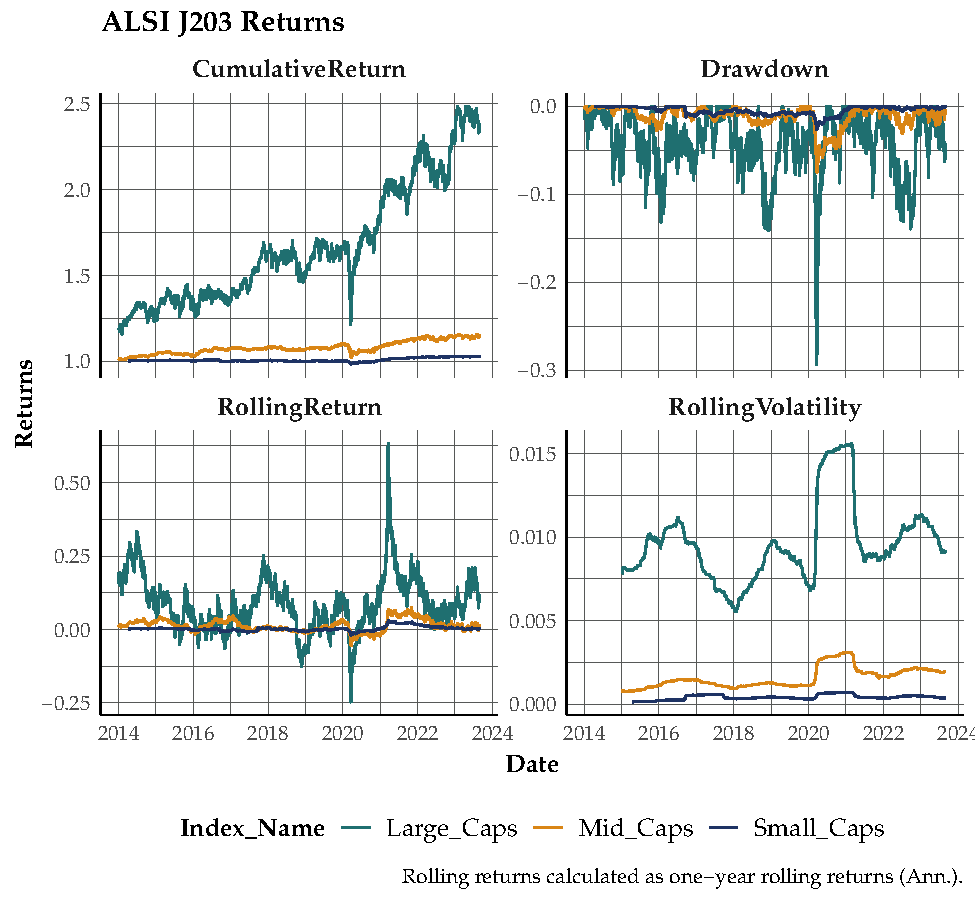
\includegraphics{Question-3_files/figure-latex/203roll-ret-1.pdf}

The second figure depicts the performance metrics for the ALSI J403
Index, broken down by market capitalization. Once again the cumulative
return chart shows that Large-Caps have yielded the highest returns over
time. The drawdown chart indicates that all market caps experience
similar declines during downturns. The rolling return graph suggests
that returns for all caps fluctuate around the same level, with no clear
consistent outperformer. Lastly, the rolling volatility graph highlights
that Large-Caps have the lowest volatility, while Small-Caps exhibit
higher volatility, with notable spikes suggesting periods of increased
market instability.

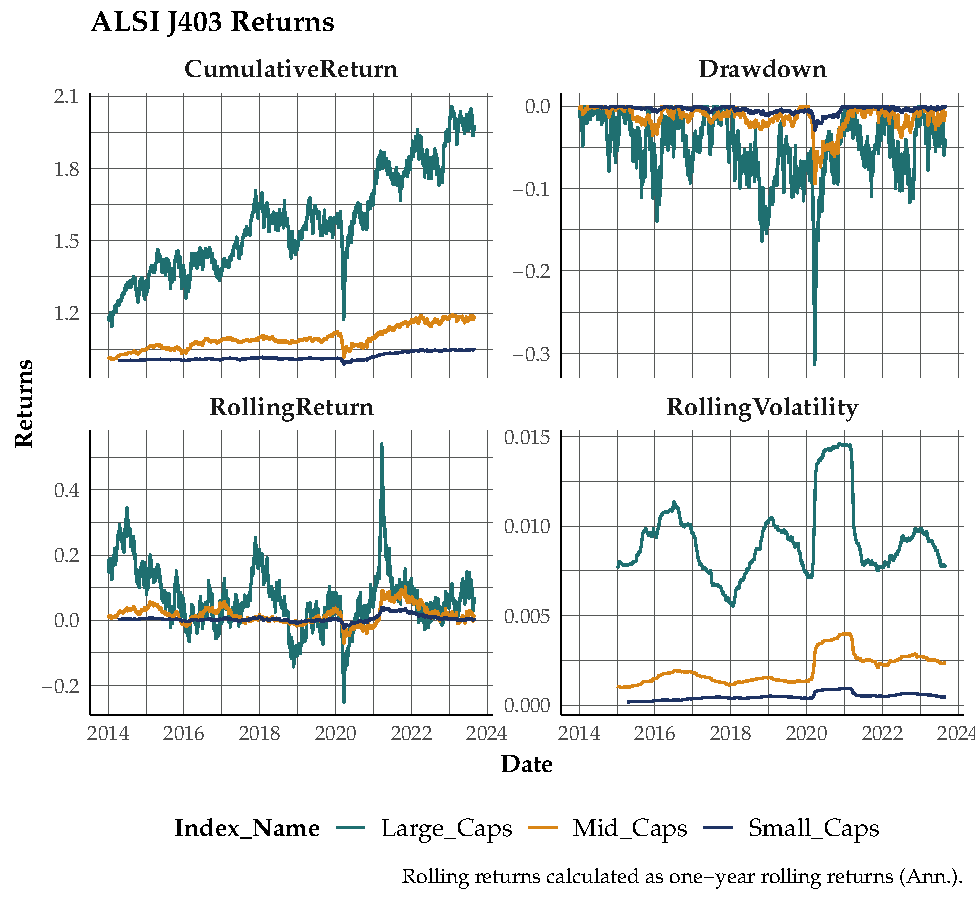
\includegraphics{Question-3_files/figure-latex/403roll-ret-1.pdf}

Comparing the two figures:

\begin{enumerate}
\def\labelenumi{\arabic{enumi}.}
\tightlist
\item
  \textbf{Cumulative Return}:

  \begin{itemize}
  \tightlist
  \item
    Both figures indicate that Large-Caps lead in cumulative returns,
    but the J203 Index seems to show a more pronounced outperformance
    relative to Mid and Small-Caps compared to the J403 Index.
  \end{itemize}
\item
  \textbf{Drawdown}:

  \begin{itemize}
  \tightlist
  \item
    Drawdown patterns are similar across both indices, with all market
    caps experiencing comparable declines during downturns. This
    suggests that market-wide events impact all caps similarly,
    regardless of the index.
  \end{itemize}
\item
  \textbf{Rolling Return}:

  \begin{itemize}
  \tightlist
  \item
    The rolling return for both indices shows that Large-Caps have more
    stable returns over time. However, the fluctuations among the caps
    are more pronounced in the J203 Index than in the J403 Index.
  \end{itemize}
\item
  \textbf{Rolling Volatility}:

  \begin{itemize}
  \tightlist
  \item
    For both indices, Large-Caps exhibit the lowest volatility. However,
    the volatility spikes for Small-Caps are more substantial in the
    J203 Index, indicating periods of increased market instability
    affecting Small-Caps more in the J203 Index compared to the J403
    Index.
  \end{itemize}
\end{enumerate}

In summary, while there are overarching similarities in the behavior of
different market capitalizations across both indices, the ALSI J203
Index displays a slightly higher differentiation between the caps,
particularly in terms of volatility and returns, suggesting a divergence
in the risk-return profile across the market caps within this index
compared to the J403.

\hypertarget{sector-exposure}{%
\section{Sector Exposure}\label{sector-exposure}}

The figure below compares the sector weightings over time for the J203
and J403 indices. In both indices, Industrials (orange) and Financials
(green) dominate the weightings, with Financials having a slightly
lesser proportion. Property (blue) and Resources (green) sectors have
smaller and relatively stable weights.

For the J203 Index, the Industrials sector has consistently the highest
weighting, followed by Financials. The J403 Index shows a similar
pattern, but with a slightly larger representation of the Resources
sector compared to J203.

Over time, the weights of each sector remain relatively stable with
minor fluctuations. There are no significant shifts or trends indicating
a change in sector composition, suggesting consistent index composition
criteria throughout the observed period. The consistent patterns across
both indices also imply similar sectoral distribution methodologies,
despite any differences in the overall index construction.

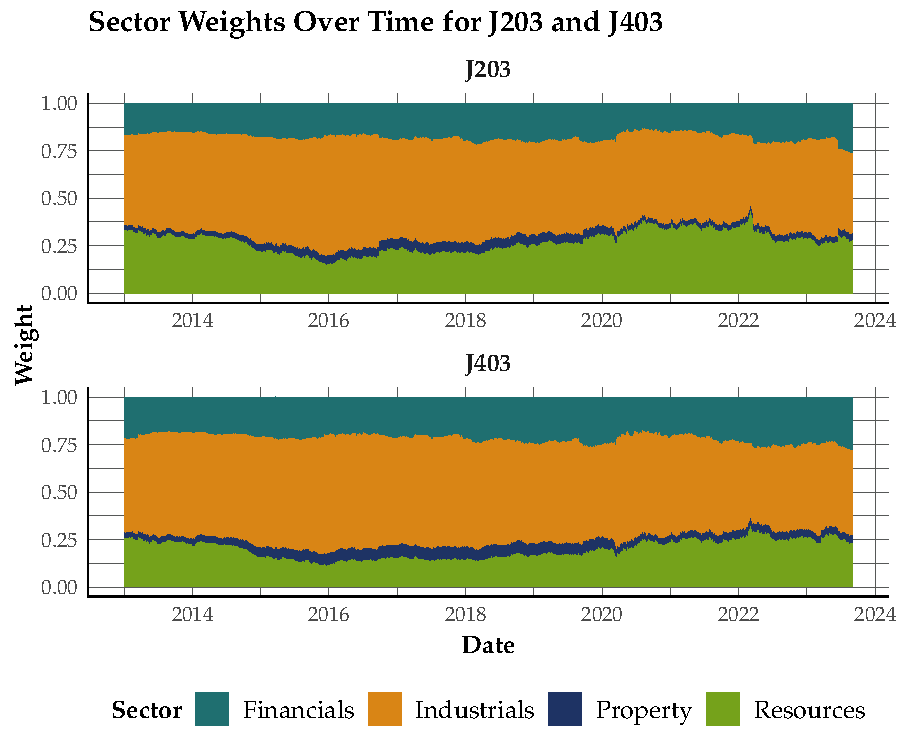
\includegraphics{Question-3_files/figure-latex/unnamed-chunk-1-1.pdf}

\hypertarget{currency}{%
\section{Currency}\label{currency}}

\begin{longtable}{lr}
\caption*{
{\large Correlation with Exchange Rate}
} \\ 
\toprule
Index & Correlation with Exchange Rate \\ 
\midrule
J203 & -0.02 \\ 
J403 & -0.06 \\ 
\bottomrule
\end{longtable}

The table above shows the correlation between the exchange rate and the
returns of the J203 and J403 indices. Both indices exhibit a negative
correlation with the exchange rate, with the J403 having a slightly more
negative correlation than the J203. This suggests that when the local
currency strengthens (exchange rate decreases), the returns on both
indices tend to decrease, but the impact is slightly more pronounced for
the J403 Index. However, the correlation values are very close to zero,
indicating a very weak relationship between exchange rate movements and
index returns for both indices.

\hypertarget{capping-unfinished-section}{%
\section{Capping (Unfinished
Section)}\label{capping-unfinished-section}}

\bibliography{Tex/ref}





\end{document}
